Supposons être en possession de $L$ et de $\mathcal{F}(L)$.
Voici comment comparer les deux automates avec Learnlib.

La classe d'automatalib util.automata.fsa.DFAs propose différentes opérations booléennes telles que la conjonction, l'équivalence, la disjonction, la disjonction exclusive, et la différence avec le vide.

Soient deux ADFs $A$ et $B$ ainsi que les langages qui sont représentés par ceux-ci, respectivement $L_A=L(A)$ et $L_B=L(B)$. 

La librairie automatalib propose, dans sa classe util.automatalib.fsa.DFAs, les fonctions suivantes :

\begin{itemize}
    \item La conjonction : $L_A\bigcap L_B$
        \begin{figure}[H]
            \center
            \colorlet{circle edge}{black}
            \colorlet{circle area}{blue!20}
            \tikzset{
                filled/.style={fill=circle area, draw=circle edge},
                outline/.style={draw=circle edge},
                whitened/.style={fill=white, draw=circle edge}}
            \def\circleA{(0,0) circle (1cm) node {$L_A$}}
            \def\circleB{(1.5,0) circle (1cm) node {$L_B$}}
          \vspace{0.6cm}
          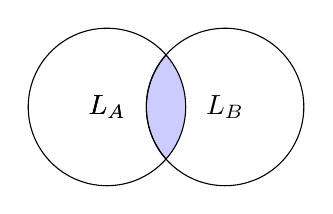
\begin{tikzpicture}
            \begin{scope}
                \clip \circleA;
                \fill[filled] \circleB;
            \end{scope}
            \draw[outline] \circleA;
            \draw[outline] \circleB;
          \end{tikzpicture}
          \caption{$L_A\bigcap L_B$ en bleu}
        \end{figure}
    
    \item L'équivalence : $L_A$ est-il égal à $L_B$ ?)
    \item La disjonction : $L_A\bigcup L_B$
        \begin{figure}[H]
            \center
            \colorlet{circle edge}{black}
            \colorlet{circle area}{blue!20}
            \colorlet{circle darker}{blue!40}
            \tikzset{filled/.style={fill=circle area, draw=circle edge},
            outline/.style={draw=circle edge}}
            \def\circleA{(0,0) circle (1cm) node {$L_A$}}
            \def\circleB{(1.5,0) circle (1cm) node {$L_B$}}
          \vspace{0.6cm}
          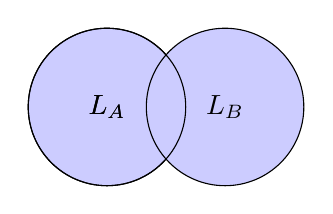
\begin{tikzpicture}
            \draw[filled]\circleA;
            \draw[filled]\circleB;
            \draw[outline]\circleA;
          \end{tikzpicture}
          \caption{$L_A\bigcup L_B$ en bleu}
        \end{figure}

    \item La disjonction exclusive ($(A\bigcup B)\backslash(A\bigcap B)$, notée $A\xor B$)
        \begin{figure}[H]
            \center
            \colorlet{circle edge}{black}
            \colorlet{circle area}{blue!20}
            \colorlet{circle darker}{blue!40}
            \tikzset{filled/.style={fill=circle area, draw=circle edge},
            outline/.style={draw=circle edge},
            whitened/.style={fill=white, draw=circle edge}}
            \def\circleA{(0,0) circle (1cm) node {$L_A$}}
            \def\circleB{(1.5,0) circle (1cm) node {$L_B$}}
          \vspace{0.6cm}
          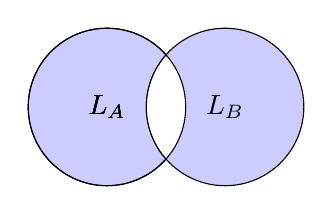
\begin{tikzpicture}
            \draw[filled] \circleA;
            \draw[filled] \circleB;
            \begin{scope}
                \clip \circleA;
                \fill[whitened] \circleB;
            \end{scope}
            \draw[outline] \circleA;
          \end{tikzpicture}
          \caption{$L_A\xor L_B$ en bleu}
        \end{figure}
    \item La différence avec le vide : $L_A \backslash \emptyset$
\end{itemize}

Toutes ces opérations sont implémentées pour les ADF. Elles sont alors implémentées en particulier pour le candidat $L$ à $AL(F)$ et pour $\mathcal{F}(L)$ qui est également un ADF.

Il est possible de comparer $L$ et $\mathcal{F}(L)$ uniquement avec ces opérations.

La comparaison est un peu plus complexe car le contre-exemple à retourner dépend de l'automate à file $F$. En effet, le contre-exemple recherché n'est pas un contre-exemple à l'égalité $L=\mathcal{F}(L)$ mais à l'égalité $L=AL(F)$.

\begin{algo}[Comparaison]
  \begin{algorithmic}[1]
    \REQUIRE $L$ et son automate $A$ ($L=L(A)$) , $\mathcal{F}(L)$ et son automate $F_A$ ($\mathcal{F}(L)=L(F_A)$) des opérations sur les automates.
    \ENSURE L'égalité en $L$ et $\mathcal{F}(L)$ ou un contre-exemple à la question $L=AL(F)$
    \IF {$L=\mathcal{F}(L)$}
        \RETURN $L$ est un point fixe de $\mathcal{F}$.
    \ELSE
        \STATE $X= L\xor\mathcal{F}(L)$ \COMMENT{$X$ est non-vide car $L!=\mathcal{F}(L)$}
        \STATE Prenons $w\in X$
        \IF {$w \in L$}
            \RETURN $w$
        \ELSE
            \IF {$w$ est une annotation valide}
                \RETURN $w$
            \ELSE
                \RETURN MOTAVANTFL($A$, $F_A$, $w$, $q_0$, $\epsilon$, faux) 
            \ENDIF
        \ENDIF
    \ENDIF
  \end{algorithmic}
\end{algo}



MOTAVANTFL est un algorithme permettant de reconstruire un mot ayant donné $w$ par l'application de la fonction $Post$. C'est son inverse. L'idée est de, pour chaque dernier $\bt$ pour un même canal $c$ et symbole $a$, explorer une autre exécution de $L$ dans lequel la barre est retirée de $\bt$. Le branchement hors du mot principal ne peut se faire qu'une fois puisqu'un seul $\theta$ est ajouté pour obtenir $w$. Cette unicité du branchement est protégée par $B$.

La branche principale, qui n'a pas bifurqué, doit être raccourcie de son dernier $\theta$ et $t_q$ doit être ajusté en conséquence.



\begin{algo}[MOTAVANTFL]
    \begin{algorithmic}[1]
        \REQUIRE
        \begin{itemize}
            \item Un ADF $A$ donnant le langage $L=L(A)$
            \item Un ADF $F_A$ tel que $L(F_A)=\mathcal{F}(L)$
            \item Un état courant $q_c$
            \item Un mot a analyser $w$
            \item Le début du mot $d$
            \item Une valeur de vérité $B$ 
        \end{itemize}
        \ENSURE un $w'$ tel que $\exists \theta, w=Post(w',\theta)$
        \STATE $S\leftarrow\emptyset$\COMMENT{l'ensemble des solutions}
        \STATE $a,w'\leftarrow w$ \COMMENT{$a$ est le premier symbole de $w$ et $w'$ le reste}
        \IF {$w'=\epsilon$}
            \RETURN $dt_{q_c}$
        \ELSE
            \IF {$|w'|=1$}
                \IF {$B$ est faux}
                    \STATE $S\leftarrow S+dt_{q_c}$
                \ELSE
                    \STATE $S\leftarrow S+dat_{q_c}$
                \ENDIF
            \ELSE
                \IF{$a\in T_Q$}
                    \RETURN $\emptyset$ \COMMENT{Car $w'$ ne serait pas correctement formatté}
                \ELSE
                    \STATE $a$ correpond à un $\theta=(p, action, q)$
                    \IF{$p=q_c$}
                        \IF{$a\in\bar{\Theta}$}
                            \STATE $\exists b=(p,action,q) \in A,\bar{b}=a$
                            \IF {$action=c!m$ et qu'il n'y a aucun $\bar{\theta}$ dans $w$ portant sur $c$ et $m$}
                                \STATE $S \leftarrow S + MOTAVANTFL(A, F_A, q, w', db, vrai)$ 
                            \ENDIF
                        \ENDIF
                        \STATE $S\leftarrow S + MOTAVANTFL(A,F_A,q,w',da,faux)$
                    \ENDIF
                \ENDIF
            \ENDIF
            \RETURN Tous les éléments de $s\in S$ correctement formattés
        \ENDIF
    \end{algorithmic}
\end{algo}

% %$dt_q$ tel que $t_q\in T_Q, \exists \theta , \theta =(q_c, action, t_q), t_q$ est un point de départ pour une transition de $F_A$.

\paragraph{Exemple d'application de MOTAVANTFL}

Soit un ADF $A$ donnant le langage $L=L(A)$. Soit un ADF $F_A$ tel que $L(F_A)=\mathcal{F}(L)$.

Considérons un appel depuis la comparaison pour le mot $w=\bt_1\bt_2\theta_3\bt_1\theta_2t_{q1} \in \mathcal{F}(L)$.

On a alors un appel sur $MOTAVANTFL(A,F_A,w,q_0,\epsilon, faux)$. 


\begin{figure}[H]
    \centering
    \begin{tikzpicture}[->,>=stealth',shorten >=1pt,auto,node distance=4cm, semithick, bend angle=10]
    \tikzstyle{every state}=[circle, scale=0.5]


    \node[state,initial]    (0) {};
    \node[state]            (1) [right of=0] {};
    \node[state]            (3) [right of=1] {};
    \node[state]            (2) [below of=3] {};
    \node[state] (4) [right of=2] {};
    \node[state] (5) [right of=3] {};
    \node[state] (6) [right of=4] {};
    \node[state] (7) [right of=5] {};
    \node[state] (8) [above of=7] {};
    \node[state] (9) [right of=6] {};
    \node[state] (10) [right of=7] {};
    \node[state] (11) [right of=8] {};
    \node[state] (12) [right of=9] {};
    \node[state] (13) [right of=11] {};

    \path [line width=2pt]
    (0) edge node {$\bt_1$} (1)
    (1) edge node {$\bt_2$} (3)
    (3) edge node {$\theta_3$} (5)
    (5) edge node {$\bt_1$} (7)
    (7) edge node {$t_q\in T_Q$} (10)
    ;
    \path
    (1) edge node {$\theta_2$} (2)
    (2) edge node {$\theta_3$} (4)
    (4) edge node {$\bt_1$} (6)
    (5) edge node {$\theta_1$} (8)
    (6) edge node {$\theta_2$} (9)
    (8) edge node {$\theta_2$} (11)
    (9) edge node {$t_q\in T_Q$} (12)
    (11) edge node {$t_q\in T_Q$} (13)
    ;
    \end{tikzpicture}
    \caption{Arbre d'exécution de MOTAVANTFL pour $w$}\label{fig:avantfl}
\end{figure}

La figure \ref{fig:avantfl} montre comment il est possible d'explorer dans $A$ tous les chemins permettant de créer un mot $w'$ tel que $\exists\theta, w=Post(w',\theta)$. Dans le cas de cet exemple, $A$ est supposé contenir toutes les transitions de \ref{fig:avantfl}. Ce n'est peut-être pas le cas. Dans ce cas, l'exploration de la branche s'arrête. 

Par le booléen $B$, on peut s'assurer de ne bifurquer qu'une fois de la branche principale, celle contenant $w$ à l'exception de son dernier symbole. En effet, bifurquer plusieurs fois donnerait un mot qui nécéssiterait plusieurs $\theta$ pour être transformé en $w$ par la fonction $Post$, ce qui n'est pas recherché.

De plus, la branche principale correspond aux $\theta$ d'envoi ou vide ($\tau$). Les branches annexes, elles, correspondent à des réceptions qui ont barré un $\theta$, d'où la scission.


